\documentclass[journal]{IEEEtran}
\usepackage[caption=false,font=footnotesize]{subfig}
\usepackage{booktabs}
\usepackage{datatool}
\usepackage{listings}
\usepackage{tikz}
\usetikzlibrary{positioning}
\usetikzlibrary{trees}
\usetikzlibrary{fit}
\usetikzlibrary{backgrounds}
\usepackage[hyphens]{url}
\usepackage{hyperref}

\lstdefinestyle{lststyle}{basicstyle=\tt\footnotesize, captionpos=b, frame=single}

\begin{document}
\DTLloaddb{keys_values}{tmp/keys-values.csv}

\title{\LaTeX\ Technical Documents with Docker and Make}

\author{Paschalis~Bizopoulos
\thanks{P. Bizopoulos is an Independent Researcher, Thessaloniki, Greece e-mail: pbizopoulos@protonmail.com}}

\maketitle

\begin{abstract}
	We propose a template for writing portable \LaTeX\ technical documents with Docker and Make in POSIX-oriented operating systems.
	The template provides a Makefile for executing the code that generates variables, tables and figures (results), which are then used during the \LaTeX\ compilation, to produce either the draft (fast) or full (slow) version of the document.
	We also present various utilities that aid in automating the results generation and increasing the reproducibility of the document.
	We release an open source repository of the template and use it to write this paper.
\end{abstract}

\section{Introduction}
Writing technical documents that present both computationally generated results (variables, tables and figures) and natural text, is one of the central aspects of computational research.
One programming paradigm that has been proposed as a solution is \textit{literate programming}~\cite{knuth1984literate} in which the author inserts snippets of code and its execution output alongside natural text.
Some applications of \textit{literate programming} include Jupyter~\cite{kluyver2016jupyter} which allows publishing code, results and explanations in a executable format, PythonTeX~\cite{poore2015pythontex} which allows Python to be executed in \LaTeX\ and ActivePapers~\cite{hinsen2014activepapers} in which code can be executed using the Java Virtual Machine.

Although \textit{literate programming} provides many advantages for demonstrative projects and immediate visual feedback during experimentation, its `dual nature' constrains authors in using specifically designed text editors thus leading to `app/vendor lock-in` situations.
Moreover this overlap between natural text and results code makes \textit{literate programming} difficult to debug and version control.

We propose a template for writing portable \LaTeX\ technical documents with Docker and Make in POSIX-oriented operating systems.
We write this paper\footnote{\url{https://github.com/pbizopoulos/latex-technical-documents-with-docker-and-make}}\footnote{\url{https://arxiv.org/abs/2005.12660}} using this template\footnote{\url{https://github.com/pbizopoulos/latex-technical-documents-with-docker-and-make-template}} and choose the Python programming language~\cite{van2007python} for generating the results.

For the rest of the paper we will refer to:
\begin{itemize}
	\item \textit{results code} as the scientific-oriented programming language code (\textit{main.py}) that produces the variables, tables and figures,
	\item \textit{results} as the variables, tables and figures that are generated by the \textit{results code},
	\item \textit{\LaTeX\ code} as the natural text (\textit{ms.tex}) and bibliography (\textit{ms.bib}),
	\item \textit{code} as both the \textit{\LaTeX\ code} and \textit{results code},
	\item \textit{document} as the technical document that contains the rendered natural text and \textit{results} and
	\item \textit{author} as the author of the \textit{document} that writes and develops the \textit{code}.
\end{itemize}

\section{Template}

\begin{figure}[!t]
	\centering
	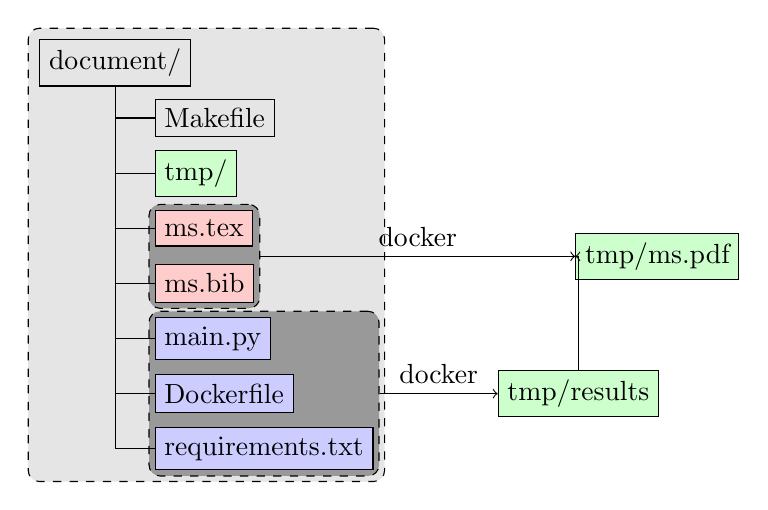
\begin{tikzpicture}[%
			grow via three points={one child at (0.5,-0.7) and two children at (0.5,-0.7) and (0.5,-1.4)},
			edge from parent path={(\tikzparentnode.south) |- (\tikzchildnode.west)}]
			\node[draw](document){document/}
			child{node[draw, anchor=west](makefile){Makefile}}
			child{node[draw, anchor=west, fill=green!20](tmp){tmp/}}
			child{node[draw, anchor=west, fill=red!20](tex){ms.tex}}
			child{node[draw, anchor=west, fill=red!20](bib){ms.bib}}
			child{node[draw, anchor=west, fill=blue!20](py){main.py}}
			child{node[draw, anchor=west, fill=blue!20](dockerfile){Dockerfile}}
			child{node[draw, anchor=west, fill=blue!20](requirements){requirements.txt}};
			\begin{scope}[on background layer]
				\node[draw, rounded corners, dashed, fill=gray!20, inner sep=4pt, fit=(document) (requirements)]{};
				\node[draw, rounded corners, dashed, fill=gray!80, inner sep=2pt, fit=(py) (requirements)](code){};
				\node[draw, rounded corners, dashed, fill=gray!80, inner sep=2pt, fit=(tex) (bib)](document){};
			\end{scope}
			\node[draw, right=1.5cm of code, fill=green!20] (results) {tmp/results};
			\path[draw, ->] (code) -- node[above]{docker} (results);
			\node[draw, right=4cm of document, fill=green!20] (pdf) {tmp/ms.pdf};
			\path[draw, ->] (results) |- (pdf);
			\path[draw, ->] (document) -- node[above]{docker} (pdf);
	\end{tikzpicture}
	\caption{The files of the template is depicted in the light gray background and the arrows denote the data flow towards generating the \textit{document}.
	Green indicates temporary cache/generated files, red \textit{\LaTeX\ code} files, blue \textit{results code} files and within the dark gray background, files that are developed by the \textit{author}.}
	\label{fig:templatefiles}
\end{figure}

\LaTeX~\cite{lamport1994latex} is a typesetting system for publishing high quality research documents, and Docker~\cite{merkel2014docker} is a container system that allows portable execution of a codebase between different operating systems/environments.

The proposed template can be used for writing \LaTeX\ \textit{documents} that present \textit{results} generated from \textit{results code} executed within a Docker container with a consistent (across different hardware, OS and programming language), minimal user interface as follows:
\begin{lstlisting}[language=bash, style=lststyle, caption={Template make options.}]
make             # Generate the draft (fast) version.
make ARG=--full  # Generate the full (slow) version.
make clean       # Remove the tmp/ directory.
\end{lstlisting}

The \textit{author} may use the template for writing \textit{documents} in the following way:
\begin{enumerate}
	\item clones the template which consists of a set of files as depicted in Fig.\ref{fig:templatefiles},
	\item specifies the name of the \textit{document} in the Makefile,
	\item creates and develops the \textit{results code} which includes:
		\begin{enumerate}
			\item \textit{main.py},
			\item \textit{Dockerfile},
			\item generating the draft and full version \textit{document} in \textit{results code} and
			\item saving \textit{results} in the \textit{tmp/} directory.
		\end{enumerate}
	\item creates and develops the \textit{\LaTeX\ code} which includes:
		\begin{enumerate}
			\item \textit{ms.tex} and \textit{ms.bib},
			\item loading \textit{results} from the \textit{tmp/} directory.
		\end{enumerate}
	\item executes \textit{make} for generating the draft version \textit{document} used during development and experimentation,
	\item executes \textit{make ARG=-{}-full} for generating the full version \textit{document} used for distribution or publication and
	\item executes \textit{make clean} to restore to a clean state by removing the \textit{tmp/} directory.
\end{enumerate}

The only restriction that the template imposes on the \textit{results code} is that the default execution should generate the draft version \textit{document} and the presence of an optional argument (-{}-full) for generating the full version.
The draft version \textit{document} (generated when calling \textit{make}) helps in faster iterations during writing and experimentation.
An example of a \textit{results code} that generates the draft version \textit{document} in the field of neural networks would be a conditional that sets the number of epochs and training/validation/test samples to a low value.

The template makes use of the automatic generation of intermediate target files of the Make program.
When the \textit{author} edits a file from \textit{results code} or \textit{\LaTeX\ code}, only the required compilation is automatically triggered with Make.
Forced compilations without change could be done using the \textit{touch} POSIX utility that updates the modification time of a file.

\section{Template utilities}
In this section we present useful utilities that can be combined with the template to automate \textit{results} generation and improve the reproducibility of the \textit{document}.

A useful \LaTeX\ package for automatically presenting variables from \textit{results} in \textit{\LaTeX\ code} is \textit{datatool} with the following example use:
\begin{lstlisting}[language=TeX, style=lststyle, caption={\LaTeX\ datatool example of loading a file that contains pairs of keys and values (tmp/keys\_values.csv) generated by a \textit{results code} and getting the value of a key named lr.}]
\DTLloaddb{keys_values}{tmp/keys_values.csv}
\DTLfetch{keys_values}{key}{lr}{value}
\end{lstlisting}

When using Python, a useful function for \textit{results code} is \textit{pandas.DataFrame.to\_latex} which automatically converts a dataframe table to a \LaTeX\ table:
\begin{lstlisting}[language=python, style=lststyle, caption={Convert Pandas DataFrame (df) to \LaTeX\ table (tmp/metrics.tex) in \textit{results code}.}]
df = pd.DataFrame(table)
df.to_latex("tmp/metrics.tex", float_format="%.2f")
\end{lstlisting}

There are some considerations need to be taken into account when reproducibility is needed.
Regarding \LaTeX\, a culprit against reproducibility is the time-date metadata embedded in the pdf output.
These can be disabled using the following commands into the \textit{\LaTeX\ code} or as extra arguments during \LaTeX\ compilation (as done by default in the template Makefile):
\begin{lstlisting}[language=TeX, style=lststyle, caption={\LaTeX\ pdf reproducibility commands.}]
\pdfinfoomitdate=1
\pdfsuppressptexinfo=-1
\pdftrailerid{}
\end{lstlisting}

Regarding the \textit{results code} for Python, random seeds need to be set to a specific value such as:
\begin{lstlisting}[language=python, style=lststyle, caption={Python reproducibility commands for some popular libraries.}]
# for build-in random module
random.seed(0)
# for numpy
np.random.seed(0)
# for tensorflow
tf.random.set_seed(0)
# for pytorch
torch.backends.cudnn.benchmark = False
torch.backends.cudnn.deterministic = True
torch.cuda.manual_seed_all(0)
torch.manual_seed(0)
\end{lstlisting}

Setting the random seeds and the previously mentioned \LaTeX\ packages, we could have deterministic stochasticity that generates the \textit{results}.

Additionally an \textit{author} can use the POSIX utility \textit{cmp} to compare \textit{documents} (generated in a different session, OS or underlying hardware) byte by byte, and diffoscope\footnote{\url{https://diffoscope.org/}} for identifying sources of non-determinism as follows:
\begin{lstlisting}[language=bash, style=lststyle, caption={Test draft document version reproducibility. This can also be used as a test script for pushed commits and pull requests to a remote repository.}]
# Generate the first draft document version
make
# Backup the first resulting pdf
cp tmp/ms.pdf tmp/ms-previous.pdf
# Update the modification timestamp of main.py
touch main.py
# Generate the second draft document version
make
# Compare draft document versions byte by byte
cmp tmp/ms.pdf tmp/ms-previous.pdf
# Compare draft document versions
# in a human readable form
diffoscope tmp/ms.pdf tmp/ms-previous.pdf
\end{lstlisting}

\section{Example use case of the template}
This section provides a use case of the template and also serves as a manual for writing \LaTeX\ \textit{documents} with Python as the \textit{results code} programming language.
We train, validate and test MobilenetV2 neural networks~\cite{sandler2018mobilenetv2} in PyTorch~\cite{paszke2019pytorch}, on MNIST~\cite{lecun2010mnist}, FashionMNIST~\cite{xiao2017fashion}, KMNIST~\cite{clanuwat2018deep}, CIFAR10~\cite{krizhevsky2009learning}, CIFAR100~\cite{krizhevsky2009learning} and SVHN~\cite{netzer2011reading}.
We use the default train, validation and test datasets and compare the use of ReLU, ReLU6\cite{dahl2013improving} and SiLU\cite{elfwing2018sigmoid} activation functions in the MobilenetV2 model.

Making use of the \textit{datatool} package the values of the following variables are not directly referred in the main \textit{.tex} file but they are instead read by an intermediate \textit{.tex} file created by the \textit{results code}: the number of epochs is $\DTLfetch{keys_values}{key}{num_epochs}{value}$, the batch size is $\DTLfetch{keys_values}{key}{batch_size}{value}$ and the learning rate for SGD is $\DTLfetch{keys_values}{key}{lr}{value}$. Additionally, making use of random seed setting we consistenly get the same figures as shown in Fig.\ref{fig:loss}, Fig.\ref{fig:kernels} and Fig\ref{fig:featuremaps}.
We also use the \textit{pandas.DataFrame.to\_latex} command which automatically converts a dataframe table to a \LaTeX\ table (as shown in Table~\ref{table:table}):

\begin{figure}[!t]
	\subfloat{\includegraphics[width=0.5\columnwidth]{tmp/MNIST-loss.pdf}}
	\subfloat{\includegraphics[width=0.5\columnwidth]{tmp/FashionMNIST-loss.pdf}}
	\caption{Comparison of MobilenetV2 with ReLU, ReLU6 and SiLU train and validation losses for MNIST and FashionMNIST.}
	\label{fig:loss}
\end{figure}

\begin{figure}[!t]
	\subfloat{\includegraphics[width=0.5\columnwidth]{tmp/CIFAR10-ReLU-kernels.pdf}}
	\subfloat{\includegraphics[width=0.5\columnwidth]{tmp/CIFAR100-ReLU-kernels.pdf}}
	\caption{The first 16 kernels of the first convolutional layer of MobilenetV2 with ReLU for CIFAR10 and CIFAR100.}
	\label{fig:kernels}
\end{figure}

\begin{figure}[!t]
	\subfloat{\includegraphics[width=0.5\columnwidth]{tmp/CIFAR10-ReLU-feature-maps.pdf}}
	\subfloat{\includegraphics[width=0.5\columnwidth]{tmp/CIFAR100-ReLU-feature-maps.pdf}}
	\caption{The first 9 feature maps of the first channel of the first convolutional layer of MobilenetV2 with ReLU for images from CIFAR10 and CIFAR100.}
	\label{fig:featuremaps}
\end{figure}

\begin{table}[h]
	\centering
	\caption{MobilenetV2 test dataset accuracies.}
	\label{table:table}
	\setlength\tabcolsep{2pt}
	\input{tmp/metrics.tex}
\end{table}

\section{Discussion}
The proposed template is based on plain text files and can be used with any POSIX-oriented operating system that supports Docker and Make.
POSIX and Make have existed for decades and have passed the test of time, while for Docker there are open standards such as the Open Container Initiative\footnote{\url{https://opencontainers.org/}} that could fill in a potential development discontinuation.
Moreover this template can be combined with any version control system, docker container registry provider and text editor thus preventing `app/vendor lock-in' situations.

Use cases of the template include:
\begin{itemize}
	\item regression testing and debugging, to ensure that changes to \textit{code} do not alter \textit{results},
	\item common development environment across multiple \textit{authors},
	\item coauthor(s), reviewers, journal editors or other researchers can easily reproduce the \textit{document} with few requirements.
\end{itemize}

\section{Conclusion}
Creation, usage and publication of technical documents are one of the top challenges for reproducible technical documents~\cite{barba2019praxis}.
The proposed template aids to this purpose by providing a way to write reproducible technical documents using the standard tools that many of the academics already use (\LaTeX, Docker, Make) in a portable, efficient and future-proof way.

\bibliographystyle{IEEEtran}
\bibliography{ms.bib}

\end{document}
